\chapter{Dialogue strategies}
\label{ch:strategies}

        This chapter sheds light on the most common way task-oriented dialogue systems manipulate concepts: slot-filling. Then several strategies that are used to get the right information from the user are presented and discussed. Finally, based on the TTP taxonomy from Chapter \ref{ch:taxonomy}, an abstract turn-taking strategy is introduced. It will be instanciated later on in the thesis.

\section{Utterance representation}
\label{sec:represent}
	
	When interacting with a dialogue system, the user's utterance can be represented in different manners. A simple way of encoding the different chunks of information that it contains is by using a slot representation. For example, if the user says \textit{I would like to buy the book Dracula by Bram Stoker}, the NLU can output the following matrix:
	
		$$
		\begin{bmatrix}
			\text{ACTION:} & \text{Buy} \\
			\text{OBJECT:} & \text{Book} \\
			\text{TITLE:} & \text{Dracula} \\
			\text{WRITER:} & \text{Bram Stoker}
		\end{bmatrix}
		$$
	
	Each entry is called a \textit{slot} and it represents a single concept in the utterance. It has two attributes: the \textit{slot name} (on the left) and the \textit{slot value} (on the right). Of course, depending on the application at hand, this matrix could be different; some slots could be considered as non relevant hence being discarded, others could be combined and new slots could be added. Therefore, while designing a dialogue system, a representation is chosen and one has to stick to it. This representation is widely used when it comes to dialogue systems design since it is a simple and natural way of representing information. It is well adapted to most tasks where the dialogue system plays the role of an interface between a user and a database. The system expects a user's request with predefined slots and depending on the latter and the database content, a response is computed and returned. This is the representation used in this thesis and Section \ref{sec:elemtask} defines it more formally.

\section{Elementary tasks}
\label{sec:elemtask}

	A \textit{task} is associated with an objective that the user wants to achieve. For example:
	
	\begin{itemize}
		\item Checking a bank account
		\item Scheduling an appointment
		\item Finding a restaurant nearby
		\item Booking a hotel room
		\item Modifying a flight reservation
	\end{itemize}
	
	Some tasks involve retrieving information from a database and others make the system modify the outside world (database modification, robot movement...). Moreover, a task can involve several \textit{elementary tasks}. An elementary task is defined as an atomic action performed by the system, after the user has made a request with all the necessary information. The task of scheduling an appointment could involve several elementary tasks, for example:
	
	\begin{enumerate}
		\item Proposing a first time window (refused by the system).
		\item Refusing a second time window that is proposed by the system.
		\item Proposing a third time window (accepted by the system).
	\end{enumerate}
	
	The way a task is organised in elementary tasks might affect the efficiency of its execution. However, this is very dependent on the task at hand and as a consequence, it is out of the scope of this thesis. The latter focuses on the way elementary tasks are handled: the optimisation of elementary tasks using different dialogue strategies.
	
	To complete an elementary task, the system requires information that can be represented as a slot matrix:
	
		$$
		\begin{bmatrix}
			slot_1 & x_1 \\
			slot_2 & x_2 \\
			... & ... \\
			slot_n & x_n
		\end{bmatrix}
		$$
	
	In this framework, a dialogue system is viewed as an automaton that is able to perform different types of elementary tasks. Hence, a dialogue is a sequence of elementary tasks: $ET_1,...,ET_k,...$. More precisely,  before performing $ET_k$, the system has to understand the user's request $X_k = (x_1, x_2, ...)$ which is a vector containing the slot values provided in her utterance (the size of the vector depends on the type of elementary task). Let $C_k$ be the dialogue context when it is time to perform $ET_k$, then $ET_k = f(X_k,C_k)$, $f$ being defined in the dialogue system. $(X_k,C_k)$ is commonly referred to as the \textit{dialogue state}.
	
	Moreover, a distinction can be made between two kinds of slots:
	
	\begin{itemize}
		\item \textbf{Constrained slots:} Some user's inputs are considered valid (but not necessarily correct) and others are not. If the slot at hand is a date and the user responds something which is not a date, this response is not valid in which case it is sure that the slot value is wrong. However, the validity of the response does not guarantee its correctness but it is noteworthy that if a generic ASR with an open grammar domain is used, valid responses that are incorrect are quite rare. On the other hand, if the ASR uses a grammar that is specific to the task at hand, they are more likely to happen.
                \item \textbf{Open slots:} Every input from the user can be considered as a valid value. For example, if the user is asked to utter a message that will be sent to some of his friends later on, he can utter anything. Therefore, unless the system asks for a confirmation, it cannot determine whether the user's input is right or wrong.
	\end{itemize}
	
	The way these slots are communicated depends on the dialogue strategy, the way the requests are formulated, the noise level and the NLU's ability to recognise a large variety of words and expressions. In Section \ref{sec:slotfillstrat}, three different slot-filling strategies are introduced and discussed.

\section{Slot-filling strategies}
\label{sec:slotfillstrat}

	Depending on the task, the dialogue system and the user, slots can be filled in different ways in order to complete an elementary task. Three generic strategies are presented here but before delving into that, the notion of \textit{initiative} is introduced. Consider the following dialogue between a customer that has just arrived to a hotel and the receptionist:
	
	\begin{dialogue}
		\speak{Customer} Hi. I would like to book a room for tonight please.
		\speak{Receptionist} Sure. Do you need a parking lot?
		\speak{Customer} No. I came here by train.
		\speak{Receptionist} All right. Would you like a smoking room?
		\speak{Customer} No, I don't smoke.
		\speak{Receptionist} Ok. What about breakfast?
		\speak{Customer} Yes, please. I will have it here.
		\speak{Receptionist} Great, all set then! Let me get your key...
		\speak{Customer} Thanks. When should I check out tomorrow?
		\speak{Receptionist} Checkout is before 11:30am.
		\speak{Customer} Ok. My train is leaving at 6:00pm, would it be possible to leave my bag here and get it back by then?
		\speak{Receptionist} Absolutely sir. No problem.
	\end{dialogue}

	This dialogue can be split into three phases. First, the customer starts the conversation by making a request. It is a result of his own initiative and he is setting the subject of the conversation. Then the receptionist provides an answer and takes the initiative right after by starting to ask specific questions. When, all the necessary information for the reservation is provided, the customer takes the initiative again to get some additional clarifications.
	
	Such a distinction can also be made in the case of dialogue systems \cite{Ferguson2007}. When using a \textit{system initiative} strategy, the latter makes requests and asks questions that the user should respond to in order to move the dialogue forward. Symmetrical strategies are called \textit{user initiative} (the user leads the course of the dialogue). Finally, strategies that involve both dialogue modes are called \textit{mixed initiative} strategies. These three dialogue strategies are presented and discussed in the following.
	
	\subsection{System initiative strategies}
	
		System initiative strategies can be compared to form-filling. The user is asked to fill several slots in a progressive way. Slot values can be asked for one by one or subset by subset. However, the \textit{one by one} case is the most common and the most simple, therefore, it will be implied when talking about system initiative strategies in the rest of this thesis.
		
		Formally, consider an elementary task $ET$ that involves $n$ slots: $slot_1, ..., slot_n$. Completing $ET$ using the system initiative strategies consists on a dialogue with $n$ system questions (dialogue acts) called $ASK(slot_1),...,ASK(slot_n)$ followed by the $n$ corresponding answers containing the required slot values $x_1,...,x_n$. However, the way errors are managed is different whether the slot at hand is open or constrained. First, it is important to note that in this thesis, the ASR is supposed to run using an open grammar (which means that most of the words in the ASR language can be recognised). So, in the case of a constrained slot, errors are easier to spot since they generally generate an invalid slot value (an information that is not of the expected type, e.g. a date when expecting a time window, a name when expecting a number, etc.). For example, if the system asks for a date and the user responds \textit{May $4^{th}$} but an ASR error occurs, then this response is more likely to be understood as some utterance which has nothing to do with a date like \textit{Mayflower} or \textit{Make lower} instead of another valid date like \textit{May $5^{th}$}. Therefore, errors are easy to spot in the case of a constrained slot (assuming that an open grammar is used for the ASR). On the other hand, as far as open slots are concerned (small message dictation, event description...), once the user provides an answer, the system has no mean of checking whether an error occured or not (since every input is valid). As a consequence, after the user provides an open slot $slot_k$, the system immediately asks for a confirmation $CONFIRM(slot_k)$ (relative to that slot only: \textit{Did you say $<$slot$>$?}). This is not the case for constrained slots and the system moves to the next question as soon as a valid answer has been provided (the only confirmation is the final one, concerning the whole elementary task).

                The example below shows a subdialogue corresponding to an elementary task with three slots, $slot_1$ and $slot_3$ are constrained whereas $slot_2$ is open (\textit{Confirmation message} refers to the last confirmation request made by the system once it collected all the necessary slot values, like \textit{Ok, so you want to book a non-smoking room for 2 nights starting from tomorrow} or \textit{You want to schedule an appointment with John on March $3^{rd}$ at 2pm. Is that right?} for example):
		
		\begin{dialogue}
			\speak{SYSTEM} $ASK(slot_1)$
                        \speak{USER} <noise>
			\speak{SYSTEM} Sorry, I don't understand. $ASK(slot_1)$
			\speak{USER} $x_1$
			\speak{SYSTEM} $ASK(slot_2)$
                        \speak{USER} $\tilde{x}_2$ (altered version of $x_2$ due to ASR imperfections)
                        \speak{SYSTEM} Sorry. $ASK(slot_2)$
                        \speak{USER} $x_2$
			\speak{SYSTEM} $ASK(slot_3)$
			\speak{USER} $x_3$
			\speak{SYSTEM} Confirmation message
                        \speak{USER} Yes
		\end{dialogue}
	
	\subsection{User initiative strategies}
	
		In this thesis, \textit{user initiative} refers to the following strategy: in order to complete an elementary task $ET$ (involving $n$ slots $slot_1,...,slot_n$), the user is supposed to provide all the slot values in a complete utterance. If there are missing slots in his request, he is asked to repeat (or reformulate) it. The dialogue then looks like this:
		
		\begin{dialogue}
			\speak{SYSTEM} What can I do for you?
			\speak{USER} $x_1$, <noise>,...,$x_n$
			\speak{SYSTEM} Sorry, I don't understand. What can I do for you?
			\speak{USER} $x_1$, $x_2$,...,$x_n$
			\speak{SYSTEM} Confirmation message
		\end{dialogue}
	
	\subsection{Mixed initiative strategies}
	
		In noisy environments, the user initiative strategy can be very tiring to the user, especially when the number of slots is important. Another way to deal with incomplete requests is to switch to the system initiative strategy to gather the missing slots, which is somehow similar to the strategy described in \cite{Lamel2000}. Suppose that the elementary task at hand $ET$ involves $n=5$ slots: $slot_1,...,slot_5$. A mixed initiative strategy dialogue looks like the following:
		
		\begin{dialogue}
			\speak{SYSTEM} What can I do for you?
			\speak{USER} $x_1$, <noise>,$x_3$,<noise>,$x_n$
			\speak{SYSTEM} $ASK(slot_2)$
			\speak{USER} $x_2$
			\speak{SYSTEM} $ASK(slot_4)$
			\speak{USER} $x_4$
			\speak{SYSTEM} Confirmation message
		\end{dialogue}

                As a side note, one can notice how the initiative strategy influences the way the information is grounded. The whole request is always grounded at the end but the system initiative and potentially the mixed initiative strategies perform separate slot grounding.
	
	\subsection{First efficiency comparison}
	
		Let $N$ be the number of turns in the dialogue that are performed to complete the elementary task $ET$ (recall that a dialogue turn is made of a system and a user turn). Also, suppose that for $ET$ to be completed, $n_s$ slots have to be specified. The objective of this preliminary study is to make a rough comparison between the previous strategies in a simple fashion, therefore, the following simplifying assumptions are made:
		
		\begin{itemize}
			\item All the slots have the same probability of not being understood: $p_{err}$.
			\item The fixed dialogue turns dedicated to greeting or saying bye for example are irrelevant for the comparison and are therefore neglected.
			\item Only constrained slots are considered (open slots are more rare and necessitate a special treatment).
			\item As a consequence, errors are mostly due to invalid input (asked for again right after the request), so the answer to the final confirmation is considered to be always positive.
		\end{itemize}

                \paragraph{System initiative:} The $i^{th}$ slot requires $N_i = 1 + n^i_{err}$ dialogue turns, $n^i_{err}$ being the number of errors that occured before the system considers that the slot value has been understood. Therefore, $N_i$ follows a geometric distribution with parameter $1-p_{err}$:

                     \begin{eqnarray}
                       \mathbb{P} (N_i = k) & = & p_{err}^{k-1} (1-p_{err}) \text{,  } \forall k \in \mathbb{N}^*
                     \end{eqnarray}

                     As a consequence, since $N = \sum_{i=1}^{n_s} N_i$:

                     \begin{eqnarray}
                       \mathbb{E} [N] & = & \frac{n_s}{1-p_{err}}
                     \end{eqnarray}

                \paragraph{User initiative:} Here, $N = 1 + n_{err}$  but $n_{err}$ corresponds to the number of user utterances where at least one slot has been misunderstood. Therefore, $N$ follows a geometric distribution with parameter $(1-p_{err})^{n_s}$ which leads to:

                     \begin{eqnarray}
                       \mathbb{E} [N] & = & \frac{1}{(1-p_{err})^{n_s}}
                     \end{eqnarray}

                \paragraph{Mixed initiative:} Let $n_{mis}$ be the number of missing (misunderstood) slots. Then by reasoning similarly as in the user initiative case,
								
											\begin{eqnarray}
												\mathbb{E} [N | n_{mis}] & = & 1 + \frac{n_{mis}}{1-p_{err}}
											\end{eqnarray}

                     Moreover, $n_{mis}$ follows a binomial distribution with parameters $p_{err}$ and $n_s$:
										
											\begin{eqnarray}
												\mathbb{P} (n_{mis} = k) & = & \dbinom{n_s}{k} p_{err}^k (1-p_{err})^{n_s-k}
											\end{eqnarray}
										
										Consequently,

                     \begin{eqnarray}
                       \mathbb{E} [N] & = & 1 + \frac{p_{err} n_s}{1-p_{err}}
                     \end{eqnarray}
										
								Figure \ref{fig:effcompare} compares the efficiency of these three slot-filling strategies with five slots and under different noise conditions. $\mathbb{E} [N]$ is used as a proxy for efficiency and $p_{err}$ represents the level of noise. It appears that the system initiative strategy is less efficient when the noise level is low compared to the user initiative one. However, as the $p_{err}$ grows, gathering the slots one by one appears to perform better. Finally, the mixed initiative strategy performs best both in low and high noise situations.
								
								\begin{figure}[t]
				\centering
				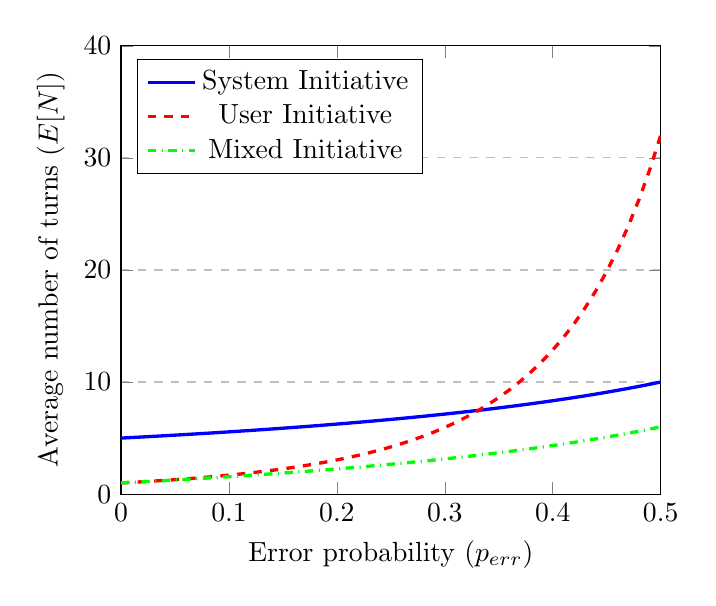
\begin{tikzpicture}[scale=1.0]
				\begin{axis}[
					xlabel={Error probability ($p_{err}$)},
					ylabel={Average number of turns ($\mathbb{E} [N]$)},
					scaled ticks = false,
					tick label style={/pgf/number format/fixed},
					xmin=0, xmax=0.5,
					ymin=0, ymax=40,
					xtick={0,0.1,0.2,0.3,0.4,0.5},
					ytick={0,10,20,30,40},
                                        legend pos=north west,
					ymajorgrids=true,
					grid style=dashed,
          %colorbrewer cycle list=Set2,
				]
				
				\addplot[color=blue,
					solid,
					very thick,
					error bars/.cd,
					y dir=both,
					y explicit,
					]
					coordinates {
					(0,5)
(0.01,5.05050505050505)
(0.02,5.10204081632653)
(0.03,5.15463917525773)
(0.04,5.20833333333333)
(0.05,5.26315789473684)
(0.06,5.31914893617021)
(0.07,5.37634408602151)
(0.08,5.43478260869565)
(0.09,5.49450549450549)
(0.1,5.55555555555556)
(0.11,5.61797752808989)
(0.12,5.68181818181818)
(0.13,5.74712643678161)
(0.14,5.81395348837209)
(0.15,5.88235294117647)
(0.16,5.95238095238095)
(0.17,6.02409638554217)
(0.18,6.09756097560976)
(0.19,6.17283950617284)
(0.2,6.25)
(0.21,6.32911392405063)
(0.22,6.41025641025641)
(0.23,6.49350649350649)
(0.24,6.57894736842105)
(0.25,6.66666666666667)
(0.26,6.75675675675676)
(0.27,6.84931506849315)
(0.28,6.94444444444444)
(0.29,7.04225352112676)
(0.3,7.14285714285714)
(0.31,7.2463768115942)
(0.32,7.35294117647059)
(0.33,7.46268656716418)
(0.34,7.57575757575758)
(0.35,7.69230769230769)
(0.36,7.8125)
(0.37,7.93650793650794)
(0.38,8.06451612903226)
(0.39,8.19672131147541)
(0.4,8.33333333333334)
(0.41,8.47457627118644)
(0.42,8.62068965517242)
(0.43,8.77192982456141)
(0.44,8.92857142857143)
(0.45,9.09090909090909)
(0.46,9.25925925925926)
(0.47,9.43396226415095)
(0.48,9.61538461538462)
(0.49,9.80392156862746)
(0.5,10)
					};
                    
                    \addplot[color=red,
					dashed,
					very thick,
					error bars/.cd,
					y dir=both,
					y explicit,
					]
					coordinates {
					(0,1)
(0.01,1.05153571281335)
(0.02,1.10629161707545)
(0.03,1.16450492244656)
(0.04,1.22643302006977)
(0.05,1.29235543489982)
(0.06,1.36257599015443)
(0.07,1.43742520951759)
(0.08,1.5172629861398)
(0.09,1.60248155139468)
(0.1,1.69350878084303)
(0.11,1.79081188001872)
(0.12,1.89490149859361)
(0.13,2.00633632832981)
(0.14,2.12572824813878)
(0.15,2.25374808871598)
(0.16,2.3911320998183)
(0.17,2.5386892155507)
(0.18,2.69730922732397)
(0.19,2.86797199079244)
(0.2,3.0517578125)
(0.21,3.24985918465773)
(0.22,3.46359406305176)
(0.23,3.69442091425689)
(0.24,3.94395579498235)
(0.25,4.21399176954733)
(0.26,4.50652102244468)
(0.27,4.82376008323414)
(0.28,5.16817865247506)
(0.29,5.542532602331)
(0.3,5.94990182661986)
(0.31,6.39373373583192)
(0.32,6.87789333714593)
(0.33,7.406721012855)
(0.34,7.98509931917638)
(0.35,8.61853037897295)
(0.36,9.31322574615479)
(0.37,10.0762109885347)
(0.38,10.9154476847742)
(0.39,11.8399760787018)
(0.4,12.8600823045268)
(0.41,13.9874949193747)
(0.42,15.2356164932545)
(0.43,16.6197972595141)
(0.44,18.1576593829952)
(0.45,19.869482337893)
(0.46,21.7786623050801)
(0.47,23.9122615317139)
(0.48,26.3016674162993)
(0.49,28.9833859145574)
(0.5,32)


					};
					
											\addplot[color=green,
					dashdotted,
					very thick,
					error bars/.cd,
					y dir=both,
					y explicit,
					]
					coordinates {
					(0,1)
(0.01,1.05050505050505)
(0.02,1.10204081632653)
(0.03,1.15463917525773)
(0.04,1.20833333333333)
(0.05,1.26315789473684)
(0.06,1.31914893617021)
(0.07,1.37634408602151)
(0.08,1.43478260869565)
(0.09,1.49450549450549)
(0.1,1.55555555555556)
(0.11,1.61797752808989)
(0.12,1.68181818181818)
(0.13,1.74712643678161)
(0.14,1.81395348837209)
(0.15,1.88235294117647)
(0.16,1.95238095238095)
(0.17,2.02409638554217)
(0.18,2.09756097560976)
(0.19,2.17283950617284)
(0.2,2.25)
(0.21,2.32911392405063)
(0.22,2.41025641025641)
(0.23,2.49350649350649)
(0.24,2.57894736842105)
(0.25,2.66666666666667)
(0.26,2.75675675675676)
(0.27,2.84931506849315)
(0.28,2.94444444444445)
(0.29,3.04225352112676)
(0.3,3.14285714285714)
(0.31,3.2463768115942)
(0.32,3.35294117647059)
(0.33,3.46268656716418)
(0.34,3.57575757575758)
(0.35,3.69230769230769)
(0.36,3.8125)
(0.37,3.93650793650794)
(0.38,4.06451612903226)
(0.39,4.19672131147541)
(0.4,4.33333333333334)
(0.41,4.47457627118644)
(0.42,4.62068965517242)
(0.43,4.77192982456141)
(0.44,4.92857142857143)
(0.45,5.09090909090909)
(0.46,5.25925925925926)
(0.47,5.43396226415095)
(0.48,5.61538461538462)
(0.49,5.80392156862746)
(0.5,6)
					};
                    

				\legend{System Initiative,User Initiative,Mixed Initiative}

				\end{axis}
				\end{tikzpicture}
				\caption{Slot-filling strategies efficiency comparison ($n_s = 5$)}
				\label{fig:effcompare}
		\end{figure}

\section{Incremental strategies}
\label{sec:incrstrat}

     Incremental dialogue processing brings a new dimension (a new degree of freedom in the decision) that can be exploited in order to improve the dialogue efficiency. In Chapter \ref{ch:taxonomy}, the following TTP have been selected for implementation: FAIL\_RAW, INCOHERENCE\_INTERP, FEEDBACK\_RAW and BARGE\_IN\_RESP from the user's and the system's perspective. In the following, the ways they can be implemented are presented.

     The concept of elementary task has been proven to be useful for slot-filling strategies analysis. As far as incremental strategies are concerned, analysis is made at a more atomic level since only one dialogue turn is considered. In the following, the user is supposed to have the floor and the system is waiting for her to provide $n_s$ slot. The DM either uses the user initiative or the mixed initiative strategy; in the system initiative strategy, the user's utterances are too short for incremental processing to be relevant.

     The reader should keep in mind that the architecture used here is the one introduced in Chapter \ref{ch:architecture}, therefore, the Scheduler module is in charge of making turn-taking decisions. Moreover, as discussed in Chapter \ref{ch:soadialogue}, another important aspect to consider is \textit{ASR instability} which is one of the major difficulties that incremental processing brings (recall that as the user speaks, his current partial utterance is not necessarily a prefix of the partial utterances to come). Nevertheless, early words in the user's utterance are more likely to stay unchanged than later ones \cite{McGraw2012}. As a consequence, making the Scheduler take decisions based on the whole current user's utterance is risky since it is likely to change. Therefore, a \textit{stability margin} (SM) is taken into account. It corresponds to the last part of the utterance that the Scheduler has to discard before making decisions. SM can be expressed in time units (discarding the last second for example) or a number of words or phonemes. The user's request without SM is called the \textit{last stable utterance}.
		
     The Scheduler can perform three kinds of actions:

     \begin{itemize}
       \item \textbf{WAIT:} Performed most of the time, it is chosen when the Scheduler decides not to retrieve the service's response at a certain micro-turn, hence waiting for the user to provide more information during the following micro-turns.
       \item \textbf{SPEAK:} The Scheduler decides to commit to the current user's utterance and to provide the corresponding service's response right away. This either translates into a barge-in or an accurate end point detection.
       \item \textbf{REPEAT:} The Scheduler does not retrieve the last service's utterance but the last pronounced of the last user's stable utterance only\footnote{This is a simple way of simulating feedback. In reality, any part of the last stable utterance could be repeated.}. The objective is not to barge-in, instead, the system performs a feedback that might trigger a reaction from the user, but not necessarily.
     \end{itemize}

     Based on these three actions, the TTP selected in Chapter \ref{ch:taxonomy} have been implemented as follows:

     \begin{itemize}

     \item \textbf{FAIL\_RAW:} If the user has been holding the floor for too long without providing a single slot value, it might be interesting for the system to interrupt her asking for a reformulation or a repeat. This situation can happen for two main reasons: the user uses off-domain words or expressions (mainly because she is not familiar with the system) or her utterance has been altered because of noise and ASR imperfections. The system can use several criteria in order to decide whether to interrupt the user or not. For example, it can rely on a time threshold: if the user speaks for a period that is larger than that threshold without providing any slot value, then it performs a SPEAK. This duration can be replaced by a number of words or phonemes for example. Consider the following dialogue where the user tries to check his bank account in a noisy environment:

          \begin{dialogue}
            \speak{USER} <noise> like to <noise> number 58 45...
            \speak{SYSTEM} ...Sorry, I don't understand. What can I do for you?
            \speak{USER} Check account number <noise> I repeat, check account 58 45 18 A.
            \speak{SYSTEM} All right, you want to check the account number 58 45 18 A right?
            \speak{USER} Yes.
          \end{dialogue}

          The user is interrupted by the system at the first dialogue turn. If the latter didn't make such a decision, its response would have been the same (\textit{Sorry, I don't understand. What can I do for you?}) since an important part of the request was lost. Therefore, the system barge-in spared the user some time and energy. In this example, the second time the user tries to formulate his request, he does it in a more concise way and repeats it as an effort to make himself clearer. This kind of behaviour has been noticed as a result of a corpus study led in \cite{Ghigi2014}.

     \item \textbf{INCOHERENCE\_INTERP:} Some user's requests can be problematic for the system because they are not coherent with the current dialogue context. The user might ask for a non existing information or try to perform some forbidden modification in the database for example. This can also be due to a transmission error (noise, ASR imperfection...) or simply because the user is not well aware of the dialogue context and the system's constraints. However, if an open grammar domain is used, the first reason is less likely to be the cause of the problem (a transmission error more often leads to a non understandable utterance by the system). Consider the following example:
		
					\begin{dialogue}
						\speak{USER} I would like to book a room for tomorrow and I will be ...
						\speak{SYSTEM} ...Sorry, we are full tomorrow.
					\end{dialogue}
					
					In this situation, it is legitimate to interrupt the user as the system is sure that the response would be the same even if it waits for the end of the request to take the floor. Implementing this behaviour is very dependent on the domain. Given the latter, a list of dialogue acts that indicate an incoherence should be identified and as soon as the service's response corresponding to the last stable utterance belongs to that list, a SPEAK should be performed.
					
     \item \textbf{FEEDBACK\_RAW:} Providing vocal feedback while the user is speaking can be very useful in some situations, especially when open slots are involved. For the sake of simplicity, only the last word of the last stable utterance is repeated in this thesis but one can go further and try to repeat any part of the user's current partial request. It is used in \cite{Skantze2009,Khouzaimi2014a} in the case of numbers dictation (see Chapter \ref{ch:architecture} for an example).
			
				However, implementing this TTP can be very challenging as the user must perceive that even though the system speaks out, it does not plan to take the floor. Moreover, negative reactions to a feedback like \textit{No, I said 45 52} must be clearly separated from positive ones. For the reasons explained in Chapter \ref{ch:taxonomy}, it will only be implemented in simulation in this thesis.
				
     \item \textbf{BARGE\_IN\_RESP (System):} When the user has provided all the necessary information for the system to provide an answer, the latter can decide to take the floor right away to improve the dialogue efficiency. The implementation of this behaviour is similar to INCOHERENCE\_INTERP. A list of dialogue acts has to be determined in advance and as soon as the service's response to the last stable utterance belongs to that list, the Scheduler decides to SPEAK.
			
     \item \textbf{BARGE\_IN\_RESP (User):} This TTP does not involve the Scheduler as the decision to speak is made by the user. However, it is important that the system does not allow user interruptions all the time, otherwise, none of the previous TTP implementations are possible. Suppose that the ASR is always listening and as soon as it detects a new input, if the system speaks, it releases the floor. Also, suppose that the user is speaking and for some reason (previous TTP), the system decides to interrupt him. During a little time window, both the user and the system are speaking and as the system is speaking it is interrupted right away. A simple solution that is adopted in this thesis is to define a time interval during which the ASR is no longer listening after the system takes the floor. Of course, this is only the case when a SPEAK is performed (the REPEAT action is not treated as such).
     \end{itemize}

     To conclude, this chapter clarified the way concepts are manipulated in most current dialogue systems as well as a few DM strategies that will be used in the following. On top of that, a few turn-taking behaviours (based on the TTP taxonomy introduced in Chapter \ref{ch:taxonomy}) and the way they can be implemented have been discussed. In the rest of this thesis, they will be instanciated in two different domains in order to form a new rule-based turn-taking strategy.
